\subsectionaddtolist{الف}

\textbf{مفهوم \lr{CQRS}:}
الگوی \lr{CQRS} (سرنام \lr{Command Query Responsibility Segregation}) به‌معنای جداسازی مسئولیت \emph{فرمان‌ها} (\lr{Commands}) که حالت سیستم را تغییر می‌دهند، از \emph{پرس‌وجوها} (\lr{Queries}) که تنها داده می‌خوانند، است:

\begin{itemize}
	\item \textbf{\lr{Command}:} نیت تغییر حالت را بیان می‌کند (مانند «این لینک را بساز» یا «این لینک را غیرفعال کن»). فرمان‌ها هیچ داده‌ای جز نتیجه‌ی موفقیت یا شکست برنمی‌گردانند.
	\item \textbf{\lr{Query}:} تنها داده می‌خواند و هیچ‌گاه حالت دامنه را تغییر نمی‌دهد (بدون اثر جانبی).
\end{itemize}

در این پیاده‌سازی، این تفکیک حتی در ساختار کد نیز آشکار است: مسیر نوشتن در بسته‌ی \lr{application/command} (هندلرهای \lr{CreateLink}، \lr{DisableLink} و \lr{RecordClick}) و مسیر خواندن در بسته‌ی \lr{application/query} (هندلرهای \lr{Redirect} و \lr{GetStats}) قرار دارد.

\textbf{دلیل استفاده از \lr{Write DB} و \lr{Read DB} مجزا:}
هسته‌ی فلسفه‌ی \lr{CQRS} این است که نیازهای سمت نوشتن و سمت خواندن ذاتا متفاوت‌اند و یک مدل واحد نمی‌تواند هر دو را به‌خوبی برآورده کند. مهم‌ترین دلایل عبارت‌اند از:

\begin{itemize}
	\item \textbf{بهینه‌سازی مستقل مدل‌ها:} مدل نوشتن باید قواعد دامنه و یکپارچگی تراکنشی را رعایت کند؛ به‌همین دلیل از \lr{PostgreSQL} رابطه‌ای استفاده شده است. مدل خواندن تنها باید سریع باشد؛ \lr{Redis} با دسترسی \lr{O(1)} برای هدایت و شمارش کلیک ایده‌آل است.
	\item \textbf{مقیاس‌پذیری ناهم‌سان:} در یک کوتاه‌کننده‌ی لینک، تعداد هدایت‌ها (خواندن) چندین مرتبه بزرگ‌تر از ساخت لینک (نوشتن) است. با دو دیتابیس می‌توان هر سمت را جداگانه مقیاس داد.
	\item \textbf{جداسازی بار (کاهش \lr{contention}):} بار سنگین خواندن، تراکنش‌های نوشتن را کند نمی‌کند و برعکس.
	\item \textbf{شکل‌دهی داده برای مصرف:} داده در \lr{Read DB} دقیقا به همان شکلی ذخیره می‌شود که پاسخ آماده باشد (نگاشت مستقیم \lr{shortCode} به \lr{longURL} و شمارنده‌ی کلیک)؛ پس در زمان خواندن نیازی به \lr{join} یا محاسبه نیست.
\end{itemize}

از آنجا که نوشتن در \lr{Write DB} و به‌روزرسانی \lr{Read DB} دو عملیات جدا هستند، \lr{Model Reader} با تأخیری کوتاه به‌روز می‌شود؛ یعنی \lr{Eventual Consistency}. این یک \lr{trade-off} آگاهانه است: در ازای کارایی و مقیاس‌پذیری بالا، می‌پذیریم که آمار کلیک یا انتشار یک لینک تازه‌ساخته‌شده با تأخیری کوتاه در سمت خواندن نمایان شود.

\vspace{0.5em}

\subsectionaddtolist{ب}

شکل~\ref{fig:components} نمودار مؤلفه‌های سامانه را نشان می‌دهد. سیستم از سه فرایند مجزا (که از یک \lr{image} واحد ساخته می‌شوند) و سه زیرساخت داده‌ای تشکیل شده است.

\begin{figure}[H]
	\centering
	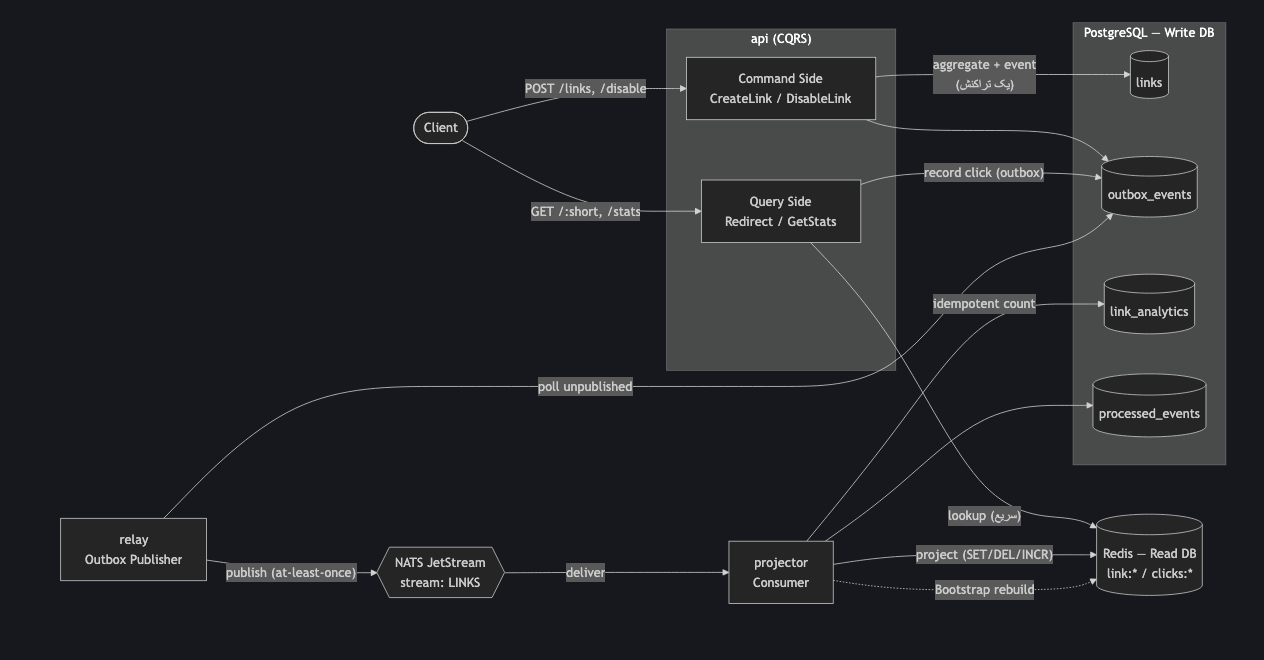
\includegraphics[width=\textwidth]{figs/component-diagram.png}
	\caption{نمودار مؤلفه‌های سامانه: تفکیک سمت نوشتن (\lr{Command}) و خواندن (\lr{Query})، الگوی \lr{Outbox}، صف \lr{JetStream} و \lr{Projector}.}
	\label{fig:components}
\end{figure}

نقش هر مؤلفه به‌صورت زیر است:

\begin{itemize}
	\item \textbf{\lr{api}:} هم سمت \lr{Command} (درخواست‌های \lr{POST}) و هم سمت \lr{Query} (درخواست‌های \lr{GET}) را سرو می‌کند، اما در کد به دو لایه‌ی کاملا جدا تقسیم شده است.
	\item \textbf{\lr{PostgreSQL} (\lr{Write DB}):} منبع حقیقت؛ شامل وضعیت \lr{aggregate}ها، جدول \lr{outbox}، شمارنده‌ی پایدار کلیک و جدول حذف تکراری.
	\item \textbf{\lr{relay}:} ردیف‌های منتشرنشده‌ی جدول \lr{outbox} را به‌ترتیب می‌خواند و روی \lr{JetStream} منتشر می‌کند (نیمه‌ی انتشار الگوی \lr{Transactional Outbox}).
	\item \textbf{\lr{NATS JetStream}:} گذرگاه پیام بادوام (با ذخیره‌سازی روی دیسک) که تحویل \lr{at-least-once} و حذف تکراری سمت‌سرور را فراهم می‌کند.
	\item \textbf{\lr{projector}:} مصرف‌کننده‌ی بادوام و \lr{idempotent} رویدادها؛ شمارنده‌ی پایدار را در \lr{PostgreSQL} و \lr{Model Reader} سریع را در \lr{Redis} به‌روز می‌کند و هنگام راه‌اندازی، \lr{Model Reader} را از روی منبع حقیقت بازسازی می‌کند.
	\item \textbf{\lr{Redis} (\lr{Read DB}):} \lr{Model Reader} سریع شامل نگاشت \lr{link:\{short\}} به \lr{longURL} و شمارنده‌ی \lr{clicks:\{short\}}.
\end{itemize}

\textbf{جریان یک عملیات کامل (هدایت و ثبت کلیک):}
شکل~\ref{fig:sequence} نمودار توالی مسیر هدایت را نشان می‌دهد. هنگام مراجعه به یک لینک کوتاه، \lr{api} ابتدا مقصد را با یک خواندن سریع از \lr{Redis} می‌یابد و بلافاصله پاسخ \lr{302} را برمی‌گرداند؛ هم‌زمان یک رویداد \lr{LinkClicked} را به‌صورت پایدار در جدول \lr{outbox} درج می‌کند. سپس \lr{relay} این رویداد را به \lr{JetStream} منتشر می‌کند و \lr{projector} آن را مصرف کرده، شمارنده‌ی پایدار را افزایش می‌دهد و مقدار به‌روزشده را در \lr{Redis} می‌نویسد. به این ترتیب مسیر داغ هدایت سریع می‌ماند و شمارش کلیک به‌صورت ناهم‌گام و بدون گم‌شدن انجام می‌شود.

\begin{figure}[H]
	\centering
	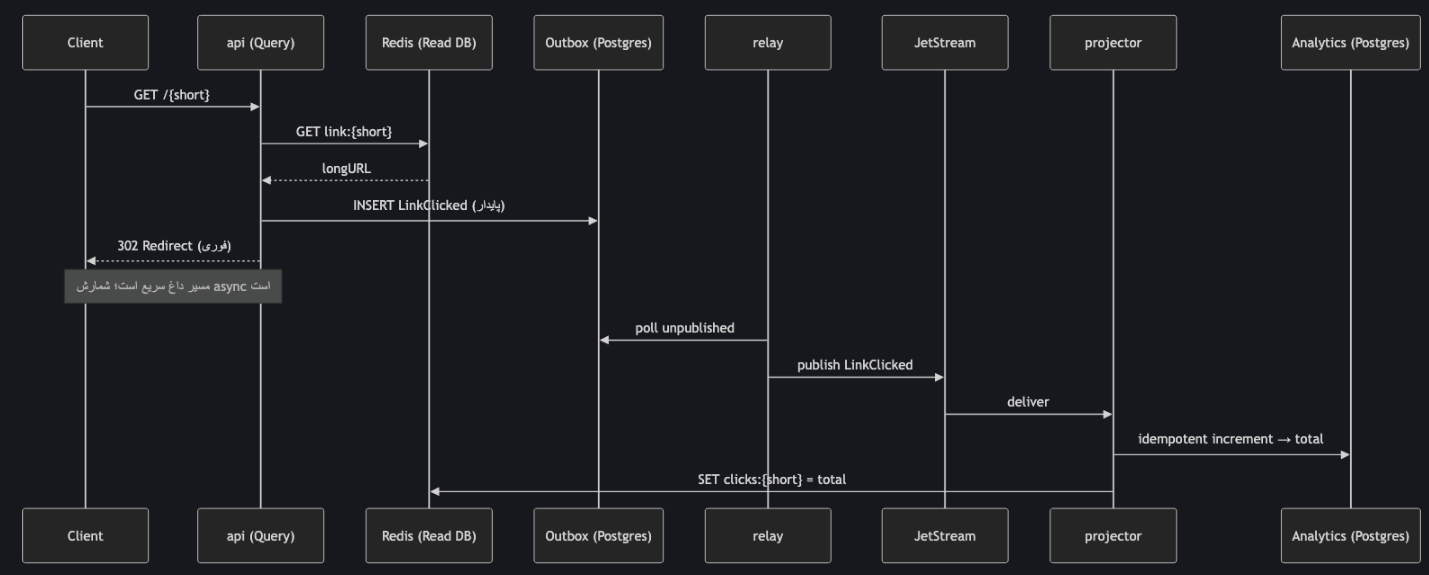
\includegraphics[width=\textwidth]{figs/sequence-diagram.png}
	\caption{نمودار توالی مسیر هدایت و ثبت کلیک به‌صورت ناهم‌گام (\lr{Eventual Consistency}).}
	\label{fig:sequence}
\end{figure}

\vspace{0.5em}

\subsectionaddtolist{ج}

\textbf{کانتینرهای سامانه:}

\begin{table}[H]
	\centering
	\begin{tabular}{|c|c|p{7.2cm}|}
		\hline
		\textbf{سرویس} & \textbf{فناوری} & \multicolumn{1}{c|}{\textbf{نقش}} \\
		\hline
		\lr{api}       & \lr{Go + Gin}        & رابط \lr{REST}؛ سمت فرمان و پرس‌وجو \\
		\hline
		\lr{relay}     & \lr{Go}              & انتشار رویدادها از \lr{outbox} به \lr{JetStream} \\
		\hline
		\lr{projector} & \lr{Go}              & مصرف رویدادها و به‌روزرسانی و بازسازی \lr{Model Reader} \\
		\hline
		\lr{postgres}  & \lr{PostgreSQL 15}   & \lr{Write DB} (منبع حقیقت) \\
		\hline
		\lr{redis}     & \lr{Redis 7 (AOF)}   & \lr{Read DB} (\lr{Model Reader} سریع) \\
		\hline
		\lr{nats}      & \lr{NATS JetStream}  & گذرگاه پیام بادوام \\
		\hline
	\end{tabular}
	\caption{کانتینرهای سامانه و نقش هر یک.}
	\label{tab:containers}
\end{table}

\textbf{مدل داده:}
جدول‌های سمت نوشتن در \lr{PostgreSQL} و کلیدهای سمت خواندن در \lr{Redis} در جدول~\ref{tab:data} آمده‌اند.

\begin{table}[H]
	\centering
	\begin{tabular}{|c|c|p{6.5cm}|}
		\hline
		\textbf{دیتابیس} & \textbf{جدول / کلید} & \multicolumn{1}{c|}{\textbf{نقش}} \\
		\hline
		\lr{Postgres} & \lr{links}            & وضعیت \lr{aggregate} (کد، \lr{URL}، وضعیت، نسخه) \\
		\hline
		\lr{Postgres} & \lr{outbox\_events}   & صف بادوام رویدادها (الگوی \lr{Outbox}) \\
		\hline
		\lr{Postgres} & \lr{link\_analytics}  & شمارنده‌ی پایدار کلیک (منبع حقیقت آمار) \\
		\hline
		\lr{Postgres} & \lr{processed\_events}& حذف تکراری برای \lr{idempotency} \\
		\hline
		\lr{Redis}    & \lr{link:\{short\}}   & نگاشت کد کوتاه به \lr{URL} اصلی \\
		\hline
		\lr{Redis}    & \lr{clicks:\{short\}} & شمارنده‌ی کلیک برای پاسخ سریع \\
		\hline
	\end{tabular}
	\caption{مدل داده‌ی سمت نوشتن و سمت خواندن.}
	\label{tab:data}
\end{table}

\textbf{الگوی \lr{Transactional Outbox} و مسئله‌ی \lr{Dual-Write}:}
اگر هنگام ساخت لینک، ابتدا در دیتابیس بنویسیم و سپس رویداد را روی صف منتشر کنیم، دو نوشتن مستقل داریم و اگر انتشار به‌خاطر کرش یا قطعی شبکه ناموفق شود، رویداد برای همیشه گم می‌شود و دو دیتابیس واگرا می‌گردند. راه‌حل این است که رویداد در \emph{همان تراکنش دیتابیسی} تغییر \lr{aggregate} در جدول \lr{outbox} نوشته شود؛ پس یا هر دو ثبت می‌شوند یا هیچ‌کدام:

\begin{lstlisting}[language=Go]
// persist aggregate state AND its events in a single transaction
return r.db.Transaction(func(tx *gorm.DB) error {
    if err := tx.Save(&model).Error; err != nil {       // aggregate state
        return err
    }
    for _, e := range events {                          // events in same TX
        if err := tx.Create(&outboxRow(e)).Error; err != nil {
            return err
        }
    }
    return nil
})
\end{lstlisting}

سپس فرایند \lr{relay} ردیف‌های منتشرنشده را خوانده و پس از انتشار موفق روی \lr{JetStream}، آن‌ها را \lr{published} علامت می‌زند. اگر \lr{relay} وسط کار کرش کند، چون ردیف هنوز علامت نخورده، در دور بعد دوباره منتشر می‌شود (تحویل \lr{at-least-once}).

\textbf{\lr{Idempotency}:}
چون تحویل \lr{at-least-once} است، ممکن است یک رویداد بیش از یک‌بار به \lr{projector} برسد. برای جلوگیری از شمارش دوباره، شناسه‌ی هر رویداد در جدول \lr{processed\_events} ثبت می‌شود و تنها در صورتی که رویداد تازه باشد، شمارنده افزایش می‌یابد؛ این کار به‌صورت یک تراکنش اتمی انجام می‌گیرد.

\textbf{پایداری و بازسازی‌پذیری:}
منبع حقیقت برای نگاشت لینک‌ها و شمارنده‌ی کلیک، \lr{PostgreSQL} با \lr{volume} پایدار است و \lr{Redis} تنها یک \lr{projection} به‌شمار می‌رود. اگر کل \lr{Redis} پاک شود، \lr{projector} هنگام راه‌اندازی با اجرای تابع \lr{Bootstrap} \lr{Model Reader} را به‌طور کامل از روی جدول‌های \lr{links} و \lr{link\_analytics} بازمی‌سازد. این رفتار به‌صورت عملی آزموده شده است: پس از اجرای \lr{FLUSHALL} روی \lr{Redis} و ری‌استارت \lr{projector}، هم نگاشت لینک‌ها و هم شمارنده‌ی کلیک‌ها دقیقا از داده‌های پایدار \lr{PostgreSQL} بازیابی شدند.

\textbf{مفاهیم \lr{DDD} به‌کاررفته:}
کل سامانه یک \lr{Bounded Context} با زبان فراگیر مشترک است و الگوهای تاکتیکی \lr{DDD} به‌صورت زیر در آن پیاده شده‌اند:

\begin{itemize}
	\item \textbf{\lr{Aggregate Root}:} موجودیت \lr{Link} ریشه‌ی تجمیع و تنها نقطه‌ی تغییر حالت لینک است؛ فیلدهای آن خصوصی‌اند و \lr{invariant} «یک لینک غیرفعال را نمی‌توان دوباره غیرفعال کرد» را خود تضمین می‌کند.
	\item \textbf{\lr{Value Object}:} مقادیر تغییرناپذیر و خوداعتبارسنج \lr{URL}، \lr{ShortCode}، \lr{LinkID} و \lr{LinkStatus}؛ مثلا \lr{URL} تضمین می‌کند که مقدار همواره یک نشانی معتبر \lr{http(s)} باشد و ورودی نامعتبر در همان مرز ساخت رد شود.
	\item \textbf{\lr{Domain Event}:} رویدادهای \lr{LinkCreated}، \lr{LinkDisabled} و \lr{LinkClicked} که «آنچه در دامنه رخ داده» را ثبت می‌کنند و مبنای به‌روزرسانی \lr{Model Reader} هستند.
	\item \textbf{\lr{Repository} (\lr{Port}):} واسط ذخیره‌سازی \lr{aggregate} در لایه‌ی دامنه تعریف می‌شود و پیاده‌سازی‌اش در لایه‌ی زیرساخت قرار دارد (وارونگی وابستگی).
	\item \textbf{\lr{Ports \& Adapters} و \lr{Persistence Ignorance}:} دامنه هیچ وابستگی‌ای به زیرساخت ندارد؛ جزئیات \lr{GORM} و پایگاه‌داده تنها در لایه‌ی \lr{infrastructure} قرار دارند و از طریق نگاشت به مدل دامنه متصل می‌شوند.
\end{itemize}
